\documentclass[paperwidth=40in,paperheight=32in,margin=1in,fontscale=0.33]{baposter}
\usepackage{amsmath}
\usepackage{amssymb}
\usepackage{enumitem}
\usepackage{subcaption}
\usepackage{float}
\usepackage{graphicx}
\usepackage[numbers]{natbib}
\usepackage{xcolor}
\usepackage{tikz}
\usepackage{pgfplots}
\usepackage[font=normalsize,labelfont=bf]{caption}


% \frenchspacing

\definecolor{box_color}{RGB}{126, 223, 231}
\definecolor{header_left}{RGB}{67, 148, 225}
\definecolor{header_right}{RGB}{77, 132, 199}
\definecolor{bg}{RGB}{215, 134, 57}


\renewcommand{\P}{\mathbb{P}}
\newcommand{\V}{\mathcal{V}}
\newcommand{\R}{\mathbb{R}}
\newcommand{\Z}{\mathbb{Z}}



\setlist{nolistsep} % more compact spacing between environments
\setlist[itemize]{leftmargin=*} % nice margins for itemize ...

\setlength{\fboxsep}{1mm}

\begin{document}
\begin{poster}{
    headerColorOne=header_left, %
    headerColorTwo=header_right, %
    boxColorOne=box_color, %
    textborder=none, %
    headerborder=none, %
    background=plain, %
    bgColorOne=bg!10, %
    %% headers
    headerfont=\Large\sf\bf, %
    headerheight=0.11\textheight, %
    headershape=rounded, %
    %% other
    columns=5,
    grid=true}{}{
	\Huge arXiv vs. snarXiv}{
	\Large Tyler Blanton and Sam Kowash\\University of Washington, Department of Physics}{
\includegraphics[height=.75in]{figures/uw_block_purple.eps}}

\headerbox{Background}{name=background,column=0,row=0,span=3}{
	The arXiv is a popular e-print repository for publications in physics, astronomy, and other quantitative sciences. It hosts nearly 1.5 million papers, of which $\sim$120,000 are in theoretical high-energy physics (\texttt{hep-th}). Physicist David {Simmons-Duffin} developed a program known as the snarXiv, which procedurally generates abstracts in the style of \texttt{hep-th} from a context-free grammar.

	Humans (even physicists) have surprising difficulty determining whether a given abstract is from the arXiv or the snarXiv. Over 750,000 guesses collected through an online sorting game, players succeeded at picking the genuine paper from a pair only 59\% of the time. Try it for yourself below!\vspace{.25\baselineskip}


	\fcolorbox{black}{white}{
	\begin{minipage}[t]{.46\textwidth}
		{\small\bf Abstract A}

		\footnotesize
		In the 20th century, a fair amount of work was done demystifying QED in the presence of a stack of canonical co-isotropic branes. In this paper, we make contact with analyzing heterotic strings, consequently reconstructing perturbation theory on $\mathbb{C}^n$, and classify anomalous dimensions in loop models with sleptons. Our computation of the solution of magnetic dualities in models of hadrons provides a certain notion of perturbation theory (taking into account cosmic rays at $\Lambda_\mathrm{QCD}$). Our results prove that decay constants turn out to be equivalent to an instanton at the Planck scale. Finally, we establish that sleptons can be brought to bear in reformulating heavy ions.
	\end{minipage}}
	%
	\fcolorbox{black}{white}{
	\begin{minipage}[t]{.46\textwidth}
		{\small\bf Abstract B}

		\footnotesize
		We study the effective action of the heterotic string compactified on particular half-flat manifolds which arise in the context of mirror symmetry with NS-NS flux. We explicitly derive the superpotential and K{\"a}hler potential at lowest order in $\alpha'$ by a reduction of the bosonic action. The superpotential contains new terms depending on the K{\"a}hler moduli which originate from the intrinsic geometrical flux of the half-flat manifolds. A generalized Gukov formula, valid for all manifolds with SU(3) structure, is derived from the gravitino mass term. For the half-flat manifolds it leads to a superpotential in agreement with our explicit bosonic calculation. We also discuss the inclusion of gauge fields.
	\end{minipage}
	}

	\vspace{0.25\baselineskip}
	We explored computational approaches to this classification problem to investigate whether its difficulty stems from snarXiv's genius, or humans' bewilderment in the face of unfamiliar jargon.
}



\headerbox{$n$-gram model}{name=ngram,column=0,row=0.41,span=2}{%
	One approach to text classification is to develop a \emph{language model}: an approximate probability distribution over word sequences or, in this case, a distribution corresponding to each class. Given a class $Y \in \{-1,1\}$ (with the negative sign referring to arXiv and the positive to snarXiv) and a document $X$ consisting of words $\{w_i\}_{i=1}^N$, we want to characterize
	%
	\begin{align*}
		\P(X | Y) &= \prod_{i=1}^N \P(w_i|w_1^{i-1}, Y),
	\end{align*}
	%
	where $w_1^{i-1}$ is the sequence of the first $i-1$ words.}


% \headerbox{Naive Bayes and likelihood-ratio classification}{name=lr,column=1,row=.8}{
% }






% \headerbox{tf--idf}{name=tfidf,column=1,row=0.0}{%
% }




\setlength{\fboxsep}{0mm}
\headerbox{Results}{name=results,column=3,row=0, span=2}{
	\vspace{-1em}
	\begin{figure}[H]
		\centering
		\fbox{\begin{subfigure}[t]{.49\textwidth}
			\centering
			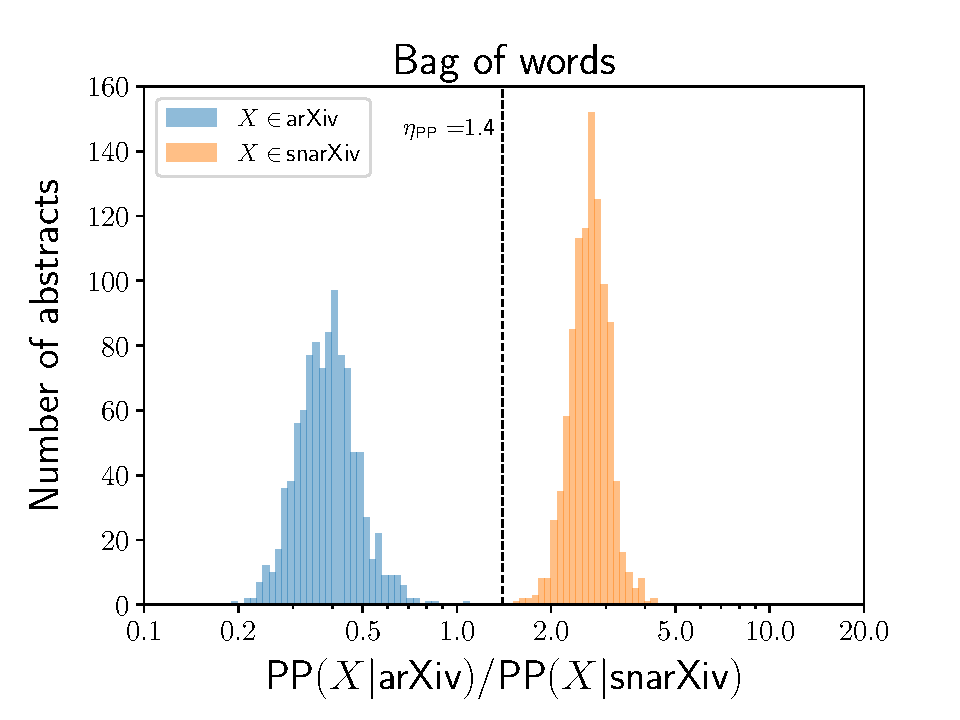
\includegraphics[width=\textwidth]{figures/BoW_histogram.pdf}
		\end{subfigure}}
		%
		\fbox{\begin{subfigure}[t]{.49\textwidth}
			\centering
			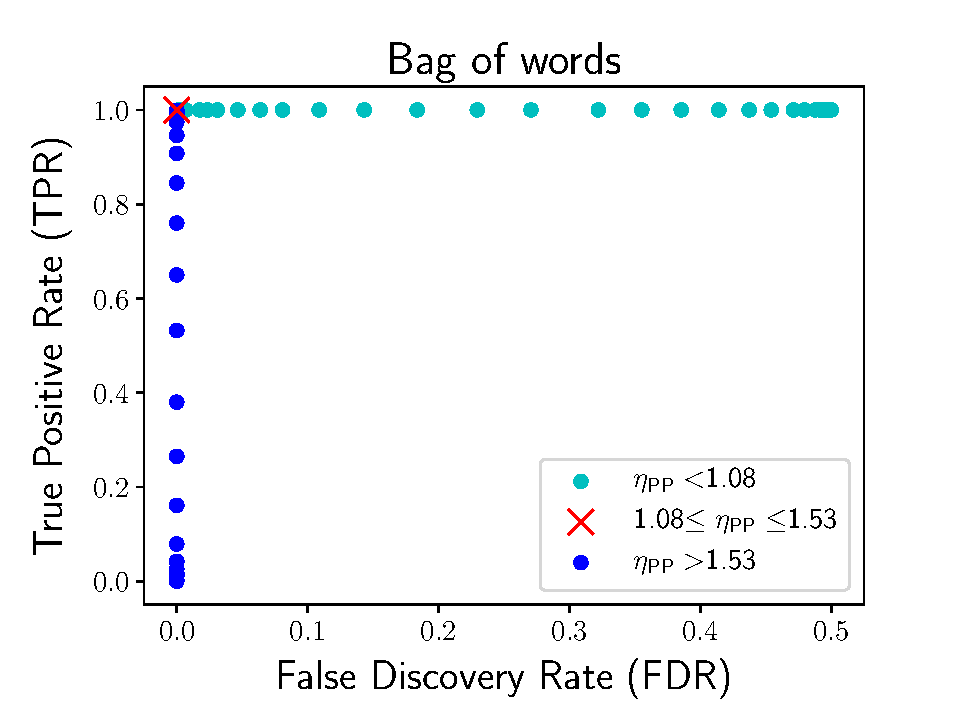
\includegraphics[width=\textwidth]{figures/BoW_TPR_FDR.pdf}
		\end{subfigure}}

		\fbox{\begin{subfigure}[t]{.49\textwidth}
			\centering
			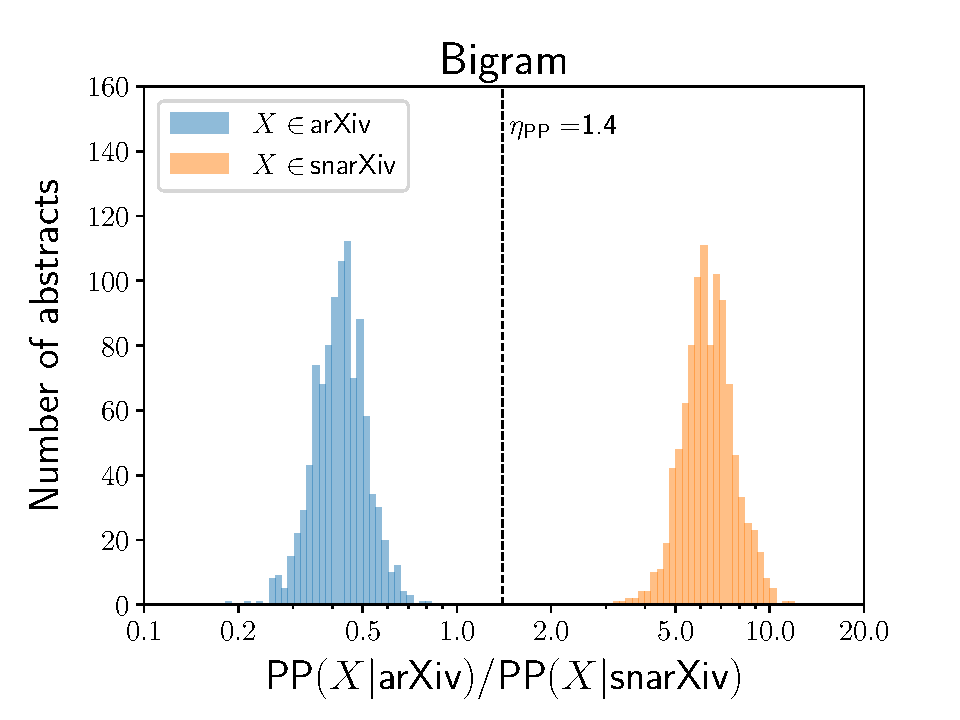
\includegraphics[width=\textwidth]{figures/bi_histogram.pdf}
		\end{subfigure}}
		%
		\fbox{\begin{subfigure}[t]{.49\textwidth}
			\centering
			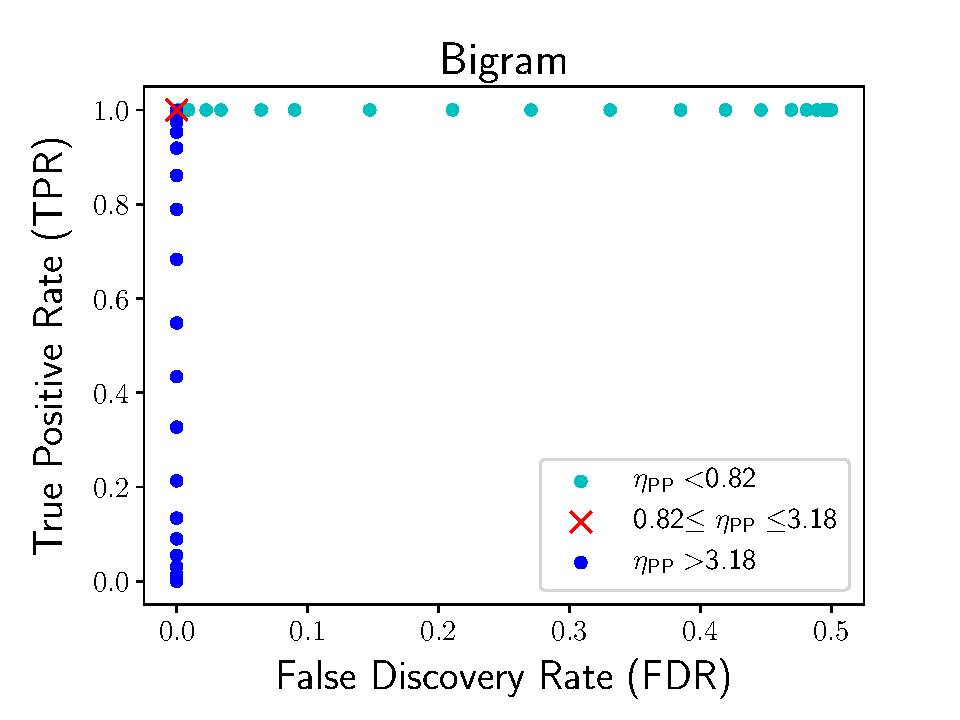
\includegraphics[width=\textwidth]{figures/bi_TPR_FDR.pdf}
		\end{subfigure}}
	\end{figure}
}
\setlength{\fboxsep}{1mm}



% \headerbox{Conclusions}{name=conclusions, column=1, row=.75}{
	
% }





% \headerbox{References}{name=refs,column=2,row=.8}{
% 	\begingroup
% 	\renewcommand{\section}[2]{}
% 	\bibliographystyle{plainnat}
% 	\bibliography{lag_paper_new}
% 	\endgroup
% }

\end{poster}
\end{document}